\chapter{Anexo I: Matriz de Consistencia}


\begin{table}[h!]
	\centering
	\small
	\begin{tabular}{ |m{5cm}|m{5cm}|m{5cm}|  }
		\hline
		\rowcolor{bluejean}
		\Centering \color{white}{PROBLEMAS}& \Centering \color{white}{OBJETIVOS}& \Centering \color{white}{HIPÓTESIS}\\
		\hline
		\rowcolor{turq}
		\Centering Problema General& \Centering Objetivo General & \Centering Hipótesis General \\
		\hline
		{\ProblemaGeneral} & { \ObjetivoGeneral} & {\HipotesisGeneral} \\
		\hline
		\rowcolor{turq}
		\Centering Problemas Específicos& \Centering Objetivos Específicos & \Centering Hipótesis Específicas \\
		\hline
		{\Pbone} & {\Objone} & {\Hone} \\
		\hline
		{\Pbtwo} & {\Objtwo} & {\Htwo} \\
		\hline
		{\Pbthree} & {\Objthree} & {\Hthree} \\
		\hline
		{\Pbfour} & {\Objfour} & {\Hfour} \\
		\hline
	\end{tabular}
	\caption{Matriz de consistencia. Fuente: Elaboración propia}
	\label{1:table}
\end{table}

\section{Árbol de Problemas}
	%\chapter*{Árbol de Problemas}
	%\addcontentsline{toc}{section}{Árbol de Problemas}
	%\renewcommand{\thechapter}{A}
	\label{anexo1}
	\begin{figure}[h]
		\begin{center}
			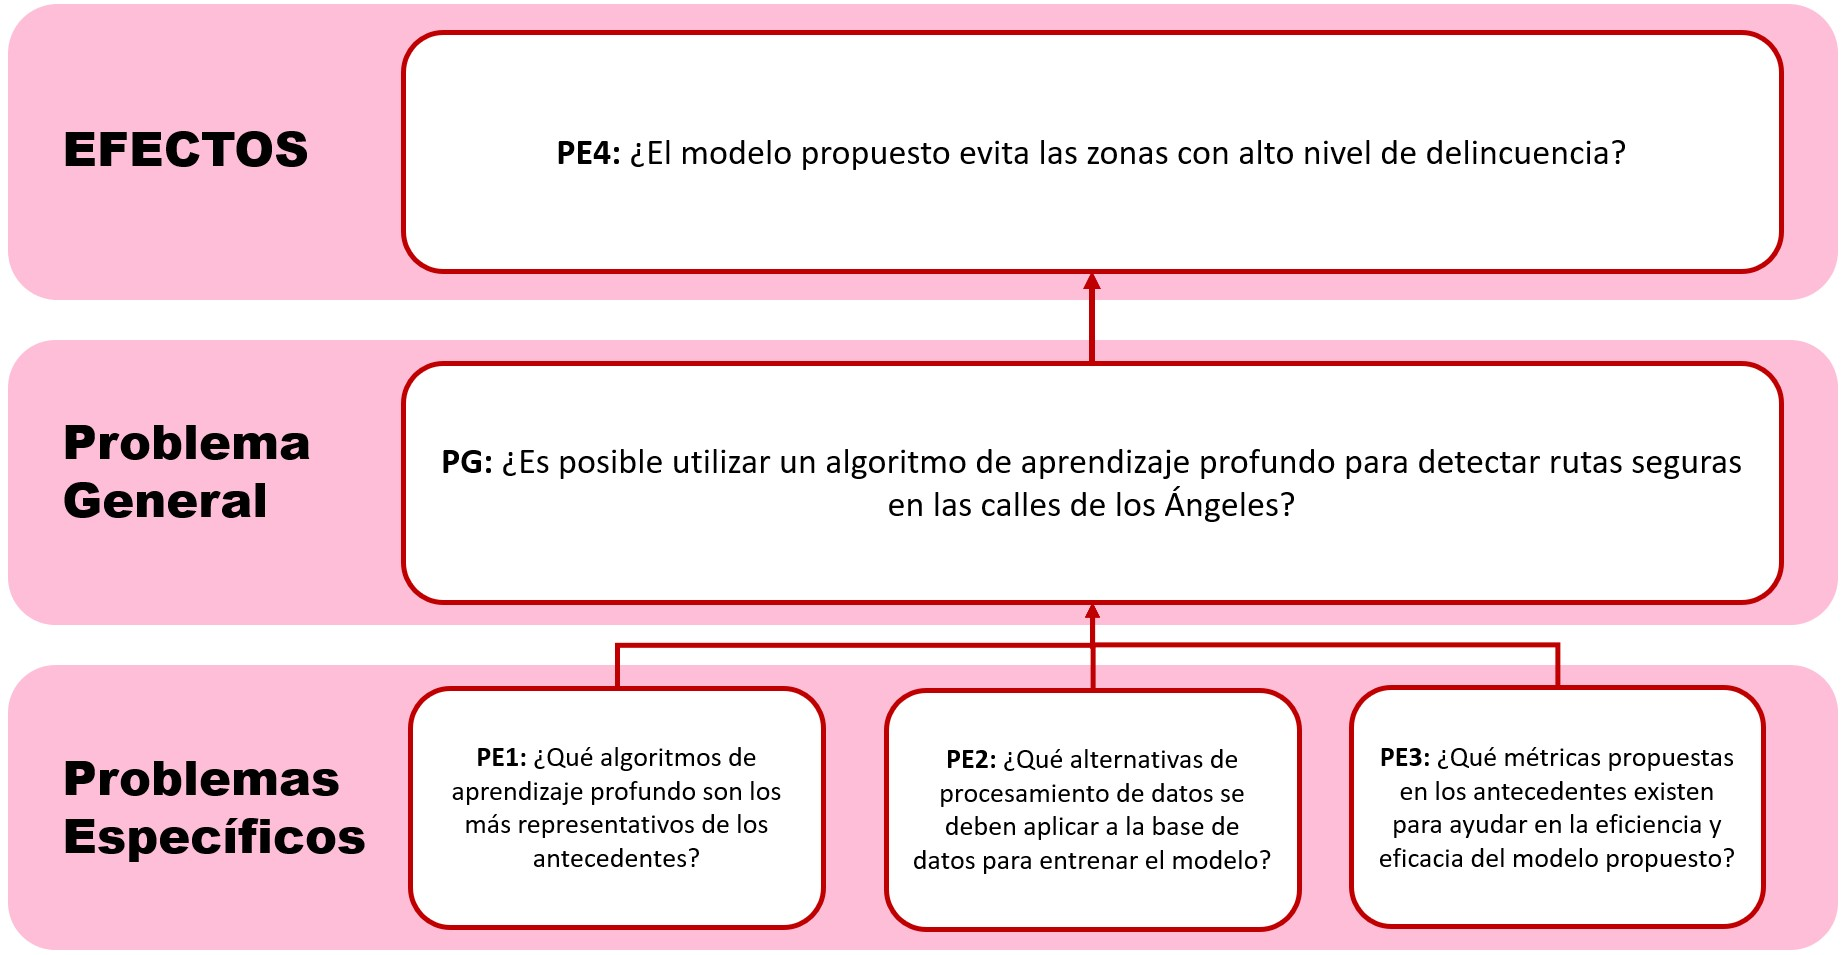
\includegraphics[width=1.05\textwidth]{anexos/PROBLEMAS.jpg}
			%\caption{Fuente: Elaboración propia}
		\end{center}
	\end{figure}
	\clearpage
	
\section{Árbol de Objetivos}
	%\chapter*{Árbol de Objetivos}
	%\addcontentsline{toc}{section}{Árbol de Objetivos}
	%\renewcommand{\thechapter}{A}
	\label{anexo2}
	\begin{figure}[h]
		\begin{center}
			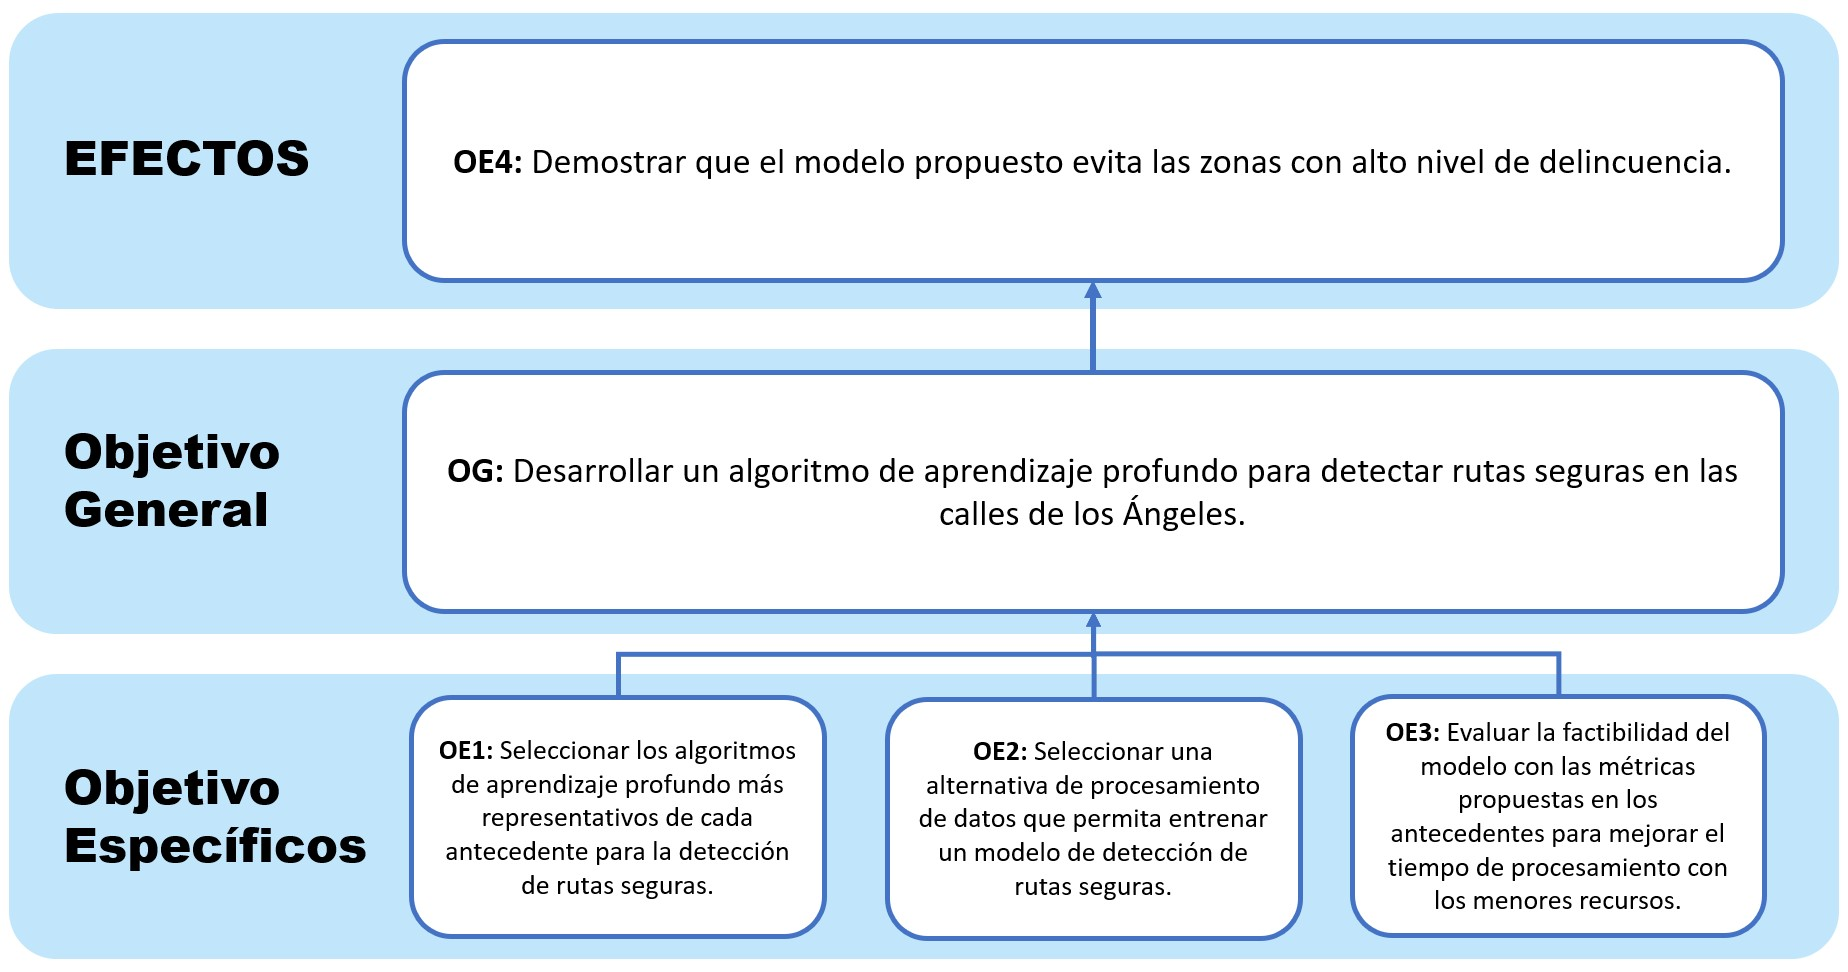
\includegraphics[width=1.05\textwidth]{anexos/OBJETIVOS.jpg}
			%\caption{Fuente: Elaboración propia}
		\end{center}
	\end{figure}
	\clearpage

\chapter{Anexo II: Resumen de Papers investigados}
%\section{Conclusiones}

\begin{table}[h]
	\newcommand{\multirot}[1]{\multirow{2}{*}[-8ex]{\rotcell{\rlap{#1}}}}
	%\scriptsize
	\footnotesize
	\centering
	\begin{tabular}{|m{0.5cm}|m{0.3cm}|m{4cm}|m{2cm}|m{0.6cm}|m{1.7cm}|m{3cm}|} 
		\hline
		\rowcolor[rgb]{0,0.251,0.502} \multicolumn{1}{|c|}{\textcolor{white}{Tipo}} & \multicolumn{1}{c|}{\textcolor{white}{N°}} & \multicolumn{1}{c|}{\textcolor{white}{Título}}                                                                             & \multicolumn{1}{c|}{\textcolor{white}{Autor}}        & \multicolumn{1}{c|}{\textcolor{white}{Año}} & \multicolumn{1}{c|}{\textcolor{white}{País}} & \multicolumn{1}{c|}{\textcolor{white}{Fuente}}                                                        \\ 
		\hline
		\multirot{Problema}                                        & 1                                             &Predicting motor vehicle theft in Santiago de Chile using graph-convolutional LSTM.                                                                               & Esquivel, N., Nicolis, O., \& Márquez, B. P                                 & 2020                                      & Chile                               & 39th International Conference of the Chilean Computer Science Society (SCCC)                                                                                      \\ 
		\cline{2-7}
		& 2                                             & SafeRoute: Learning to navigate streets safely in an urban environment                                                            & Levy, S., Xiong, W., Belding, E., \& Wang, W. Y.                     & 2020                                        & USA                                  &ACM Transactions on Intelligent Systems and Technology (TIST)                                                \\ 
		\hline
		\multirow{2}{*}[-14ex]{\rotcell{\rlap{Propuesta}}}
		& 3                                             & Route-the safe: A robust model for safest route prediction using crime and accidental data.                           & Soni, S., Shankar, V. G., \& Chaurasia, S.                             & 2019                                        & India                                          & Int. J. Adv. Sci. Technol                                                                    \\ 
		\cline{2-7}
		& 4                                             & Real-time deep reinforcement learning based vehicle navigation                                                                                & Koh, S., Zhou, B., et al.                                          & 2020                                        & Reino Unido                                          & Applied Soft Computing                                                             \\ 
		\hline
		\multirow{4}{*}[-28ex]{\rotcell{\rlap{Técnica}}}                                          & 5                                             & Algoritmo para calcular la ruta más segura y óptima                   & Cano, S., \& Tabares, S. A. A.                                      & 2022                                       & Colombia                                        & OSF Repository  \\ 
		\cline{2-7}
		& 6                                             & A reinforcement learning-based routing algorithm for large street networks. International Journal of Geographical Information Science                                                    & Li, D., Zhang, Z., Alizadeh, B., et al.          & 2024                                        & USA                                        & International Journal of Geographical Information Science              \\ 
		\cline{2-7}
		& 7                                             & Real-time safest route identification: Examining the trade-off between safest and fastest routes & Ghoul, T., Sayed, T., \& Fu, C.             & 2023                                        & Canada                                         & Analytic methods in accident research              \\ 
		\cline{2-7}
		& 8                                             & Análisis y desarrollo de modelos de predicción de links en redes mediante técnicas de Deep Learning.  & Muñoz, A.                                    & 2022                                        & España                                          & Archivo Digital UPM                           \\
		\hline
	\end{tabular}
	\caption{Cuadro Resumen de Papers investigados. Fuente: Elaboración propia}
\label{A:table}
\end{table}




